\ca{\chapter{Implementation}}
\renewcommand{\baselinestretch}{\mystretch}
\label{chap:Impl}
%\setlength{\parindent}{0pt}

\PARstart{\ca{S}}{\ca{everal}} \ca{%
implementations of various portions of the final optimised controller application were developed independently, so that each portion can be verified working before integration. The implementations were developed as the following steps:
}

\begin{enumerate}[noitemsep,leftmargin=4cm]
  \item[Qt2 demo:] A controller specific application using C++ with Qt2-based GUI, to test the performance of the NP1380 platform and showcase an interactive application design.
  \item[\texttt{VixenLinky}:] C\# implementation of a controller specific application, for use as the references of the optimal performances on different platforms.
  \item[Playback engine:] Integrate the sequence decoding routine from \texttt{VixenLinky} to the Vixen application as a separate playback engine.
  \item[\texttt{VixenConsole}:] A command-line interface (CUI) version of the Vixen application, but with only minimal functionalities and a working playback engine for embedded platforms.
  \item[Video transcoding:] Various programs for video processing, integrated into the playback engine for video format support.
\end{enumerate}

\clearpage

\section{\ca{Qt2-based} implementation}

A GUI application dedicated to the \texttt{TCPLinky} controller was developed using C++ as \ca{a user-friendly alternative implementation} showcase. This application was developed specific to the Noah NP1380 platform listed in \sref{sec:systems}. This device is a handheld embedded device based on a 10 years old SoC chip, originally designed for educational use \ca{such as electronic dictionaries}. Fortunately, this devices uses Linux system and Qt2 as GUI. Therefore, it is possible to test Vixen application on this low-end platform.

\begin{figure}[t]
  \centering
  \includegraphics[width=0.45\textwidth]{Figs/vixen_noah.png}%
  \caption{\footnotesize Screenshot of Vixen Qt2 demo on Noah NP1380}
  \label{fig:vixen_noah}
\end{figure}

\fref{fig:vixen_noah} shows a screenshot of the dedicated application. The method of performance profiling through statistic files in proc file system was also tested. These smaller progress bars at the lower half of the application shows percentages of CPU time spent on different tasks, such as user space applications, kernel mode and interrupt handling. Most of the time only less than $50 \%$ CPU time was used for this controller application, \ca{indicating that} even this low-end device is capable of handling thousands of lighting channels.

\section{Minimal C\# implementation}

To set up a reference baseline for optimal performance, sequence rendering application \ca{named \texttt{VixenLinky} was developed. It was implemented using C\#, takes} the same \ca{``Raw''} sequence data \ca{format}, but \ca{supports} only the \texttt{TCPLinky} controller developed in \sref{sec:tcplinky}. \ca{It was} implemented as \ca{simply} as possible without all intermediate layers \ca{and module loading routines}, but still \ca{using} a threading structure \ca{identical to} the original Vixen application. \ca{The source code for controlling the \texttt{TCPLinky} controller} was ported directly from the original Vixen application \ca{to ensure compatibility and similarity}.

With this program, the \ca{ideal} performance \ca{of the new playback engine} on each platform can be measured. The \ca{remaining performance limitation factors are} sequence loading performance and controller update speed. Therefore, options to unlimit the update interval of both sequence loading and controller update were added separately \ca{for the measurements of maximum update rates}.

\fref{fig:vixenlinky_noah} shows an example of performance data gathered on the Noah NP1380 platform through \texttt{VixenLinky} using \ca{the exported test sequence}. The refresh rates of both playback and controller \ca{were} very stable around \ca{the configured} 50 fps. The CPU usage \ca{peaked} at $60.0 \%$\ca{,} while most of the time it \ca{was} distributed around $20.0 \%$ and $30.0 \%$ (first and third quartiles).

\begin{figure}[!t]
  \centering
  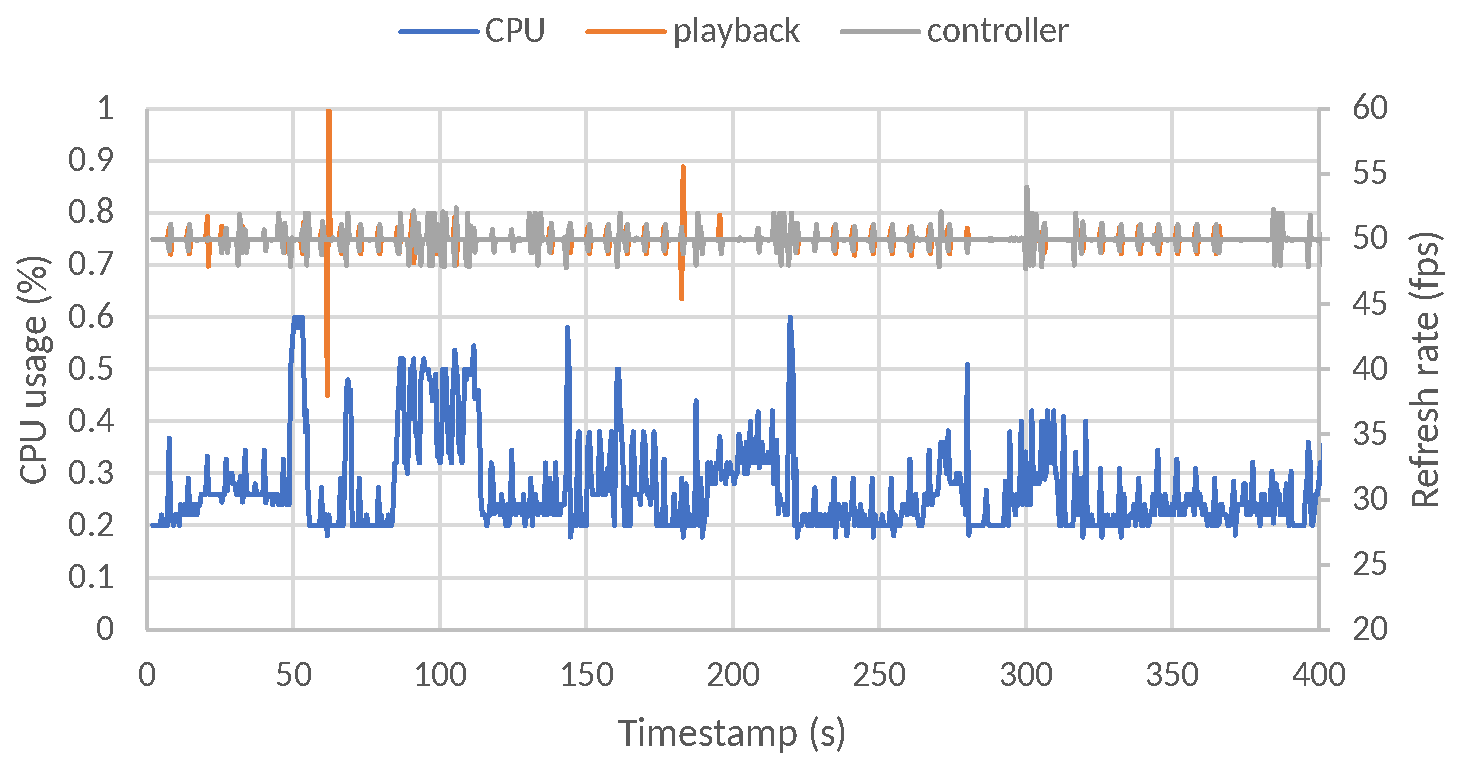
\includegraphics[width=0.8\columnwidth]{Figs/vixenlinky_noah.eps}
  \caption{\footnotesize Performance of \texttt{VixenLinky} on Noah NP1380}
  \label{fig:vixenlinky_noah}
\end{figure}

\section{Playback engine}

\subsection{Implementation}

After \ca{verifying} the ability \ca{to load and render} the exported lighting \ca{sequences} by controller specific \ca{applications}, the C\# code for loading exported sequence \ca{from \texttt{VixenLinky}} was integrated into Vixen application as a separate playback engine.

Several code branches were added to switch between the original execution engine and the new playback engine. The execution engine was still used as the default engine to simplify status checking and support the sequence editor. The playback engine will be switched to \ca{only if an exported sequence was loaded to it and started rendering}.

The playback engine starts by reading the exported network XML file. To simplify the process, \ca{an} XML object serialiser was used to interpret \ca{and store} the XML \ca{data structure} to a similarly structured C\# object for later access. The information \ca{read} from XML will be used to determine controller channel mapping, update interval and optional audio media file. To further reduce \ca{matching} overhead, the controller names will be looked up and converted to their unique ID (GUID) \ca{instead}. The optional audio media file was supported by utilising the same audio media functions from original execution engine.

All preview, element and filter updates were skipped in the playback engine. The translation layers were skipped, since the sequence data is already specific to the controllers. However, in order to match the existing interface of controller modules, \ca{segments of sequence data frame buffer} still need to be copied again \ca{as command batches for each controllers}, incurring some unnecessary overhead.

The structure of update management was also changed\ca{, as illustrated in \fref{fig:update}}. \ca{In the original execution engine}, the application updates \ca{data buffers} from \ca{controller update requests}, which requires the use of mutex \ca{locks to coordinate} data \ca{accesses} between controller threads. With a configuration \ca{consists} of multiple controllers, potential lock contention of the mutex can also incur some overhead. \ca{To address this issue, another} thread dedicated to sequence loading was \ca{added} to the playback engine, similar to the structure of controller specific implementations. In this way, only the sequence loading thread may update the channel data buffer, \ca{removing} the need of mutex \ca{locks}.

\begin{figure*}[t]
  \centering
  \subfloat[Execution engine]{\frame{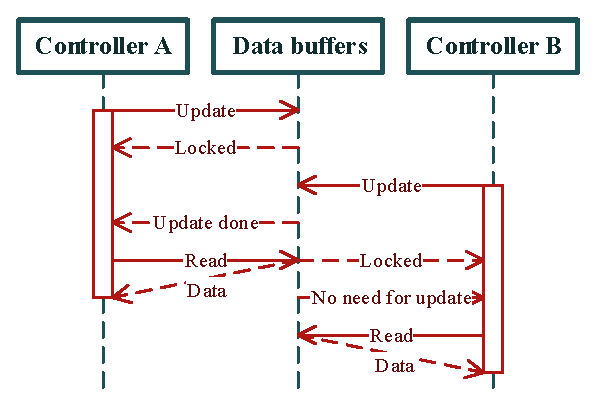
\includegraphics[height=4cm]{Figs/update_execution.eps}}}
  \hfil
  \subfloat[Playback engine]{\frame{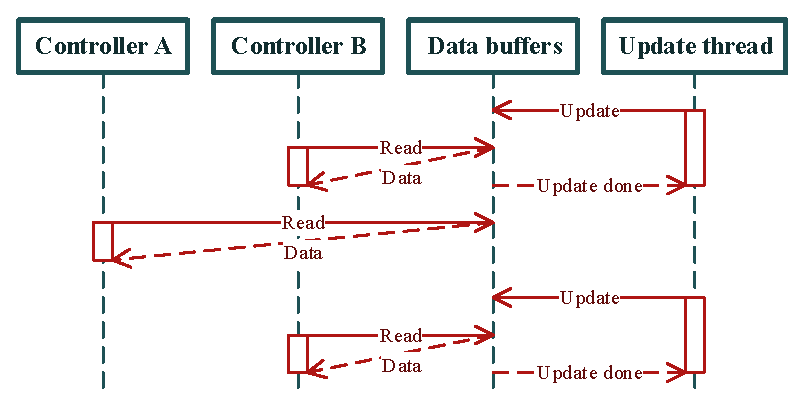
\includegraphics[height=4cm]{Figs/update_playback.eps}}}
  \caption{\footnotesize Update management of Vixen engines}
  \label{fig:update}
\end{figure*}

One major drawback of using the playback engine is that the \ca{exported} data cannot be mapped back to element states yet\ca{, which is essentially the reverse of export}. Therefore, editing the \ca{exported} sequence using the built-in editor and the preview output were not supported.

\subsection{Integration}

A simple control dialog was added as a menu entry for the \ca{new playback} engine, as shown by \fref{fig:vixen_playback}. More complex and user-friendly UI design is possible, however, due to limited time \ca{constraints} this control dialog should be sufficient for this project and proof of concept.

\begin{figure}[t]
  \centering
  \includegraphics[width=0.8\columnwidth]{Figs/vixen_playback.png}
  \caption{\footnotesize Screenshot of the playback engine control dialog}
  \label{fig:vixen_playback}
\end{figure}

The playback control was also integrated \ca{as a new type of action into the} built-in schedulers. It can therefore be scheduled to execute at specific \ca{times with different sequences}, possibly \ca{together with other existing actions including} schedules using the original execution engine. The new playback engine does not need additional pre-process for show schedules, \ca{and} can be directly started within seconds.

\subsection{Performance}

\fref{fig:playback} shows the performance of the \ca{new} playback engine \ca{on the same Microsoft Windows-based platform} using \ca{an exported} ``Raw'' sequence. At the first and the last few seconds, the playback engine stopped, the original execution engine was used instead during idle state. However, the execution engine still uses around $30 \%$ of CPU time during idle. But as soon as playback started, CPU usages drops to around $6 \%$ with stable refresh frame rates.

\begin{figure}[t]
  \centering
  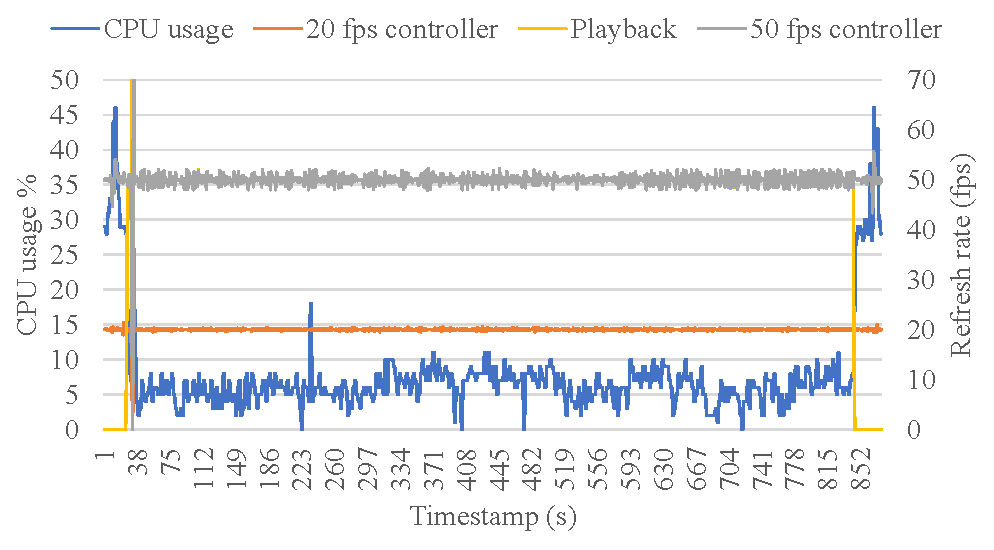
\includegraphics[width=0.8\columnwidth]{Figs/playback.eps}
  \caption{\footnotesize Performance of the new playback engine on Microsoft Windows}
  \label{fig:playback}
\end{figure}

\section{Console application}

\subsection{Implementation}

\ca{To improve the usability of the new playback engine on Linux-based platforms especially embedded platforms, a} Command-line User Interface (CUI) version of Vixen, named \texttt{VixenConsole}, was implemented. It is easier to operate and manage a CUI based program through remote connection \ca{and automated scripts} instead of a distorted partially functional GUI application \ca{on Linux}. \cref{chap:Guide} \ca{lists} the detailed usage description of \texttt{VixenConsole}.

\ca{Different from the reference implementation \texttt{VixenLinky} that only supports the \texttt{TCPLinky} controller, this \texttt{VixenConsole} application is a simplified version of the Vixen GUI application, supports all controller modules the Vixen GUI application supports.}

The original core codebase from \texttt{Vixen.dll} was used in this program with some necessary modifications. Instead of full initialisation from Vixen GUI application, only \ca{available controllers modules and their configurations} will be \ca{loaded during start-up by} \texttt{VixenConsole} to reduce overheads. In this way, the code for the playback engine, module and data loading is \cad{still} shared with the Vixen GUI application, \ca{can also receive} future improvements and patches.

\texttt{VixenConsole} reads configurations from the same location as Vixen application, the \texttt{Vixen 3} folder from user home directory. All configurations are stored as XML files, exported directly from settings object using XML serialiser. The ability to list available controllers and their configurations \ca{was} added to \texttt{VixenConsole}. However, configuration modification was not yet possible from \texttt{VixenConsole}, due to the complexity of supporting every \ca{possible} types of configuration fields within the project time constraint. To create or modify the configuration, the Vixen GUI application can be used from a computer running Microsoft Windows. Editing the XML configuration files directly using text editors is also possible.

The \texttt{FMOD} plugin used by the Vixen GUI application was outdated, \ca{and} no longer available for download.

\cmt{Therefore, audio playback using the ``Raw'' sequence was unsupported by \texttt{VixenConsole}.}

\ca{
The \texttt{VixenConsole} application does not have a build-in show scheduler. Instead, existing job scheduler utilities such as \texttt{crontab} \cite{crontab} can be used, since the \texttt{VixenConsole} application with the new playback engine does not have a pre-rendering step, therefore can be started within a reasonable amount of time. Together with the help of Linux shell scripting, this way of scheduling can be much more flexible than a fixed time scheduler. To reduce start-up time, back-to-back playback of multiple sequences were also supported.
}

\subsection{Loading performance}

On an embedded platform with limited computation power, the loading time of \texttt{VixenConsole} and all controller modules can take a significant time. The implemented \texttt{tidy} operation can reduce a small portion of the loading time, by remove unused settings for elements and filters\ca{, which} also reduces the size of XML \ca{configuration files}.

However, it still takes \ca{about 30 seconds} from starting \texttt{VixenConsole} to \ca{be able to render} on the \ca{Raspberry Pi B+} platform\ca{, in contract to only 5 seconds on the Raspberry Pi 3B platform}. This loading time is for the mono runtime to preform some necessary tasks such as dynamic \ca{recompilation}, \ca{and is} unavoidable.

\subsection{Execution performance}

\fref{fig:raw-seq-p-c} compares the performance between \texttt{VixenLinky} and \texttt{VixenConsole} on multiple platforms. The performance comparison was done by \ca{unlimiting} the playback and controller refresh rate separately using both \texttt{VixenLinky} and \texttt{VixenConsole} applications\ca{;} a total of \ca{four} tests on each of the platforms. The refresh rate data over the entire sequence time \ca{is} then summarised \ca{using} a five-number summary representation, i.e. sample minimum, lower quartile, median, upper quartile and sample maximum. The mean values were also plotted as points. The refresh rate axis is log scale, to focus on the lower performance figures over all platforms.

\begin{figure}[t]
  \centering
  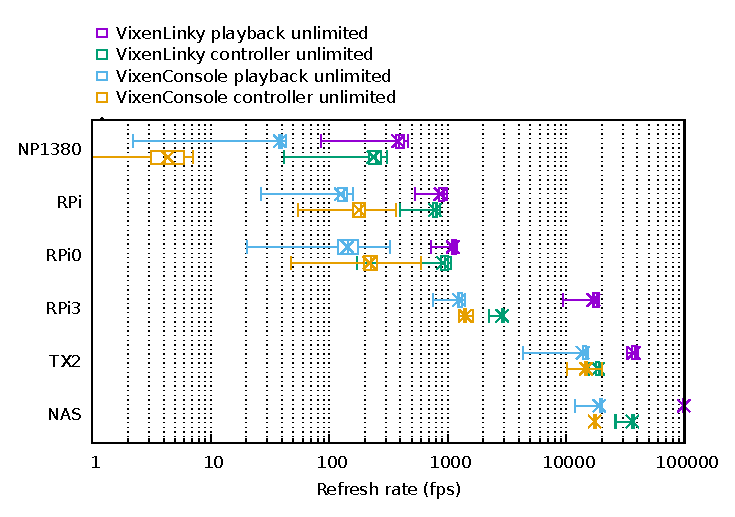
\includegraphics[width=0.9\textwidth]{Figs/raw-seq-p-c.eps}
  \caption{\footnotesize Performance comparison between \texttt{VixenLinky} and \texttt{VixenConsole}}
  \label{fig:raw-seq-p-c}
\end{figure}

By separating playback and controller update tests, the two major performance limitation factors of file IO and processing power can be separately tested.

The figure shows \ca{that} \texttt{VixenConsole} runs a few times slower than the minimal implementation \texttt{VixenLinky}. On NP1380, the controller refresh rate drops below 10 fps, unusable for a 50 fps sequence. It still performs adequately on Raspberry Pi B+\ca{;} both the maximum possible playback and controller refresh rate were significantly higher than 50 fps.

The mono profiler was used in an attempt to \ca{further optimise the \texttt{VixenConsole} application} on Raspberry Pi B+ platform. However, it was not particularly \ca{successful}. As shown by \lref{lst:mono_sample}, \ca{there are not any significant performance optimisation opportunities available. The} thread sleeping method, \ca{IO read} methods and update methods are all \ca{mandatory and} just as expected. Some overheads from copying command arrays do show up on the summary as array coping functions, but they are \ca{insignificant, also} unavoidable for controller module interface compatibility.

\begin{lstlisting}[float,floatplacement=ht,language=,label=lst:mono_sample,captionpos=b,caption={\footnotesize Summary of time spent in each method, collected by mono profiler}]
Method call summary
Self(ms)   Calls Method name
 584540   38673 System.Threading.Thread:SleepInternal (int)
 520043    2604 System.IO.InotifyWatcher:ReadFromFD (intptr,byte[],intptr)
 410638   21047 System.Threading.WaitHandle:WaitOne_internal (intptr,int)
  63712   19119 Vixen.Sys.Playback:ReadFrame ()
  56368   21044 VixenModules.Output.TCPLinky.TCPLinky:UpdateState (int,Vixen.Commands.ICommand[])
  18617   41132 System.IO.MonoIO:Read (intptr,byte[],int,int,System.IO.MonoIOError&)
  16052  114460 object:__icall_wrapper_ves_icall_array_new_specific (intptr,int)
  12287   49221 System.Array:FastCopy (System.Array,int,System.Array,int,int)
  11344   21044 System.Net.Sockets.Socket:Send_internal (intptr,byte[],int,int,System.Net.Sockets.SocketFlags,int&,bool)
   7274    3020 System.Runtime.CompilerServices.RuntimeHelpers:SufficientExecutionStack ()
\end{lstlisting}

\section{Video data format}

With the implementation of \texttt{VixenConsole}, the process of designing and pre-rendering (exporting) the sequence on Vixen application then playback later using \texttt{VixenConsole} became very similar to the process of video editing and playback. Therefore, it \ca{was thought to} be beneficial to add support for video sequence format.

\subsection{Implementation}

The open source \texttt{ffmpeg} framework \cite{ffmpeg} was used for video processing. The open source nature ensures up-to-date version of \texttt{ffmpeg} is available on all testing platforms.

The \texttt{ffmpeg} framework uses the C programming language for its API. The complicity of different data structures used by \texttt{ffmpeg} results in no up-to-date C\# wrapper API available for use directly. Therefore, an intermediate wrapper layer between Vixen and \texttt{ffmpeg} was developed to encapsulate all complex \texttt{ffmpeg} routines using C.

The development of video integration was separated into multiple steps. Firstly, several C programs were developed to test individual video processing functions including video encoding, video decoding, stream muxing and metadata \ca{retrieval}. Afterwards, working code segments were combined into a dynamic library, with a simplified API suitable for C\#. A C\# wrapper class was then developed using the \texttt{InterOp} service \cite{interop}, together with another C\# program for testing video encoding and decoding. After all these small testing programs had been confirmed working, the C\# wrapper was finally integrated into Vixen with the playback engine. The playback engine checks for \ca{the} input file extension to determine whether to load the file as \ca{an} exported ``Raw'' sequence or \ca{a} video file.

To ensure lossless transcoding from the ``Raw'' sequence to \ca{a} video stream, the transcoding programs were tested by encoding example sequences to \ca{videos} then decoded back to \ca{new sequences}. The \ca{new} sequences were then compared for any difference \ca{to the original sequence}, using the GNU \texttt{diff} tool \cite{diff}. Makefile was used for automated \ca{compilation} and testing.

To minimise number of files needed for playback, the optional audio file was muxed together with the video stream, and the network configuration XML file was stored directly as \ca{a} string literal in \ca{a} video metadata field \ca{named} ``comment'', as shown by \fref{fig:video-info}.

\begin{figure}[t]
  \centering
  \includegraphics[width=0.7\textwidth]{Figs/video_info.png}
  \caption{\footnotesize Media information of an example video sequence}
  \label{fig:video-info}
\end{figure}

In the playback engine, video frames will be transformed to controller data frames for rendering. However, the existing audio rendering engine \texttt{FMOD} from Vixen only supports media file playback. The required functionality of playing decoded data frames was not available from its C\# API. To resolve this issue, C code for operating a newer version of \texttt{FMOD} was added to the wrapper library. The playback engine transfers the decoded audio frame back to the wrapper library for audio playback.

It is possible to support audio playback with exported ``Raw'' sequences using the newer version of \texttt{FMOD}. However, this was not implemented yet.

\cmt{TODO: Implement audio playback with ``Raw'' sequence, update performance data}

\subsection{Benefits and limitations}

The first noticeable benefit was reduction in sequence file size. The ``Raw'' sequence format was implemented without any compression algorithm, \ca{and} always has a size linear to total sequence time and channel count. The video formats reduced the sequence size to around $\nicefrac{1}{10}$ of the ``Raw'' sequence. \tref{tbl:size} compares file sizes in different formats of the same example sequence.

\begin{table}[t]
  \centering
  \begin{tabular}{l|l|l}
    \hline
    \textbf{Type} & \textbf{Sequence size} & \textbf{With audio} \\
    \hline
    Editable sequence                                 & 8.88 MiB  & 24.4 MiB  \\ \hline
    50 fps exported \texttt{Raw} sequence             & 337 MiB   & 352 MiB   \\ \hline
    50 fps \texttt{rgb24} encoded video (lossless)    & 26.6 MiB  & 42.5 MiB  \\ \hline
    50 fps \texttt{yuv444p} encoded video (lossless)  & 26.6 MiB  & 42.5 MiB  \\ \hline
    50 fps \texttt{yuv420p} encoded video (lossy)     & 18.2 MiB  & 34.1 MiB  \\ \hline
  \end{tabular}
  \caption{\footnotesize File size comparison of different formats}
  \label{tbl:size}
\end{table}

Using the video format, the exported sequence, audio and configuration information are combined into a single file. This reduction of file count can sometimes simplify the management and sharing of multiple sequences. However, an unexpected limitation on metadata length was encountered on Raspberry Pis. The \texttt{libav} fork of \texttt{ffmpeg} provided by the raspbian distribution of version \texttt{jessie} has an arbitrary limitation of 1000 characters for metadata field length, not enough for all XML configuration information. To work around this issue, some inactive fields of the XML configuration was removed for Raspberry Pis. To completely remove this issue, newer version of \texttt{ffmpeg} without this limitation can be compiled for Raspberry Pis.

The \texttt{yuv420p} encoded video listed in \tref{tbl:size} were transcoded from the \texttt{rgb24} encoded video using the \texttt{ffmpeg} command-line tool. It is possible to add support for multiple video formats as options to the developed video library to directly transcode from ``Raw'' sequence to other video formats. However, this can make the encoding process over complicated. Instead, other dedicated video transcoding tools can be used for the same task. The decoding routine used in playback engine was designed to support any video encoding format, by converting the video frames to \texttt{rgb24} format internally. This is another benefit of using a video file. All tools developed for general purpose video processing, editing and filtering can also be used for the exported sequences.

With these sophisticated video \ca{compression} algorithms, a drop of the sequence loading speed was expected. Fortunately, the \texttt{ffmpeg} library is capable of utilising media acceleration features to speed up video decoding, such as SIMD instructions and dedicated video decoding hardware. However, a \ca{low} resolution video, such as the $76 \times 76$ video from \fref{fig:video-info}, is more than capable of supporting thousands of controller channels. It may not leverage the full advantage of dedicated high resolution hardware video decoding accelerators.

\subsection{Encoding formats}

\begin{figure*}[t]
  \centering
  \subfloat[\texttt{rgb} channel order]{\includegraphics[width=0.3\textwidth]{Figs/video/rgb24-raw-scale.png}%
  \label{fig:video-rgb}}\hfil
  \subfloat[\texttt{yuv} channel order]{\includegraphics[width=0.3\textwidth]{Figs/video/yuv-scale.png}%
  \label{fig:video-yuv}}\hfil
  \subfloat[\texttt{yuvp} channel order]{\includegraphics[width=0.3\textwidth]{Figs/video/y-u-v-scale.png}%
  \label{fig:video-yuvp}}\\
  %\subfloat[Constant rate factor 6]{\includegraphics[width=0.3\textwidth]{Figs/video/rgb24-6-scale.png}}\hfil
  %\subfloat[Difference blend]{\includegraphics[width=0.3\textwidth]{Figs/video/rgb24-6-scale-diff.png}}\hfil
  %\subfloat[XOR blend]{\includegraphics[width=0.3\textwidth]{Figs/video/rgb24-6-scale-xor.png}}\\
  \subfloat[Constant rate factor 12]{\includegraphics[width=0.3\textwidth]{Figs/video/rgb24-12-scale.png}}\hfil
  \subfloat[Difference blend]{\includegraphics[width=0.3\textwidth]{Figs/video/rgb24-12-scale-diff.png}}\hfil
  \subfloat[XOR blend]{\includegraphics[width=0.3\textwidth]{Figs/video/rgb24-12-scale-xor.png}}\\
  \subfloat[Constant rate factor 24]{\includegraphics[width=0.3\textwidth]{Figs/video/rgb24-24-scale.png}}\hfil
  \subfloat[Difference blend]{\includegraphics[width=0.3\textwidth]{Figs/video/rgb24-24-scale-diff.png}}\hfil
  \subfloat[XOR blend]{\includegraphics[width=0.3\textwidth]{Figs/video/rgb24-24-scale-xor.png}}\\
  %\subfloat[Constant rate factor 24]{\includegraphics[width=0.3\textwidth]{Figs/video/yuv444p-24-scale.png}}\hfil
  %\subfloat[Difference blend]{\includegraphics[width=0.3\textwidth]{Figs/video/yuv444p-24-scale-diff.png}}\hfil
  %\subfloat[XOR blend]{\includegraphics[width=0.3\textwidth]{Figs/video/yuv444p-24-scale-xor.png}}\\
  \subfloat[\texttt{yuv420p} encoding]{\includegraphics[width=0.3\textwidth]{Figs/video/yuv420p-0-scale.png}%
  \label{fig:video-420}}\hfil
  \subfloat[Difference blend]{\includegraphics[width=0.3\textwidth]{Figs/video/yuv420p-0-scale-diff.png}%
  \label{fig:video-420-diff}}\hfil
  \subfloat[XOR blend]{\includegraphics[width=0.3\textwidth]{Figs/video/yuv420p-0-scale-xor.png}%
  \label{fig:video-420-xor}}\\
  \caption{\footnotesize Video encoding formats comparison of frame 13850}
  \label{fig:video-pix_fmt}
\end{figure*}

There are several possible ways to encode sequence channel data into a video pixel format. \fref{fig:video-rgb}, \ref{fig:video-yuv} and \ref{fig:video-yuvp} shows 3 different channel orders tested.

For the \texttt{rgb} format, channel data was copied line-by-line into a video frame buffer with \texttt{rgb24} pixel format. The channel data fills sequentially the red, green and blue channels of continuous pixels, also called packed format.

Similarly, \fref{fig:video-yuv} was encoded as packed \texttt{yuv} for comparison. However, only planar pixel format of \texttt{yuv444} is available for video frames. The frame buffer stores an entire frame of \texttt{y} channel first, followed by a frame of \texttt{u} and \texttt{v} channels. For the packed \texttt{yuv} format, this requires complex buffer copying routine, \ca{which} may decrease the performance.

\fref{fig:video-yuvp} shows the appearance of storing channel data as planar \texttt{yuv} format \ca{instead}. Because the example sequence contains lots of \texttt{RGB} elements, pixels with similar colours were all separated by two other pixels in the planar format. This separation resulted in lots of sharp pixel boundaries, which can be badly degraded when transcoding to lower quality video settings.

The second and third rows of \fref{fig:video-pix_fmt} show the quality degradation with lower quality settings using the same \texttt{rgb24} pixel format. The increase of the constant quality factor (CRF) means the video data rate will be more restricted and reduced. The frame difference of CRF 12 is hardly visible, but the \texttt{XOR} blend clearly shows there are binary differences to the reference frame.

Within the 3 formats tested, \texttt{yuv420p} probably is the most common video encoding format currently. It is also more commonly supported by hardware video accelerators. However, \texttt{yuv420p} is not capable to store channel data losslessly with the same image resolution. It is more suitable for storing realistic videos, where sudden colour changes between pixels are uncritical and not common. Colour degrade and cross-talk between channels are unavoidable with the \texttt{yuv420p} encoding format, as shown by the last row of \fref{fig:video-pix_fmt}.

\cmt{Insert data table about file sizes, data rates and PSNR \wn{16}}
